\documentclass[12pt]{report}
\usepackage{tikz}
\usepackage{parskip}
\usepackage{mathtools}
\usepackage{flexisym}



\begin{document}
\newcommand\tab[1][1cm]{\hspace*{#1}}

%title page
\author{Andre Gregoire}
\title{CIS770 Homework 2}
\maketitle

%problem 1
\textbf{ Problem1}\newline
\textit{1.1.}\newline
\begin{center}
	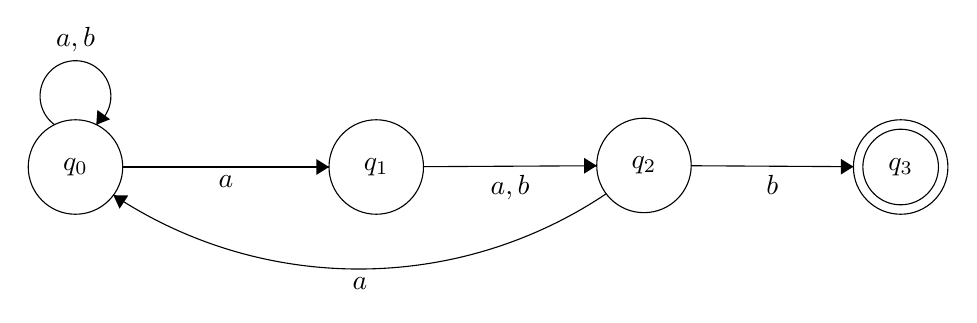
\begin{tikzpicture}[scale=0.2]
		\tikzstyle{every node}+=[inner sep=0pt]
		\draw [black] (16.9,-15.6) circle (3);
		\draw (16.9,-15.6) node {$q_0$};
		\draw [black] (36,-15.6) circle (3);
		\draw (36,-15.6) node {$q_1$};
		\draw [black] (53,-15.5) circle (3);
		\draw (53,-15.5) node {$q_2$};
		\draw [black] (69.3,-15.6) circle (3);
		\draw (69.3,-15.6) node {$q_3$};
		\draw [black] (69.3,-15.6) circle (2.4);
		\draw [black] (15.577,-12.92) arc (234:-54:2.25);
		\draw (16.9,-8.35) node [above] {$a,b$};
		\fill [black] (18.22,-12.92) -- (19.1,-12.57) -- (18.29,-11.98);
		\draw [black] (19.9,-15.6) -- (33,-15.6);
		\fill [black] (33,-15.6) -- (32.2,-15.1) -- (32.2,-16.1);
		\draw (26.45,-16.1) node [below] {$a$};
		\draw [black] (39,-15.58) -- (50,-15.52);
		\fill [black] (50,-15.52) -- (49.2,-15.02) -- (49.2,-16.02);
		\draw (44.5,-16.06) node [below] {$a,b$};
		\draw [black] (56,-15.52) -- (66.3,-15.58);
		\fill [black] (66.3,-15.58) -- (65.5,-15.08) -- (65.5,-16.08);
		\draw (61.15,-16.06) node [below] {$b$};
		\draw [black] (50.602,-17.3) arc (-56.16114:-123.52143:28.215);
		\fill [black] (19.31,-17.39) -- (19.7,-18.25) -- (20.25,-17.41);
		\draw (34.97,-22.58) node [below] {$a$};
	\end{tikzpicture}
\end{center}


\textit{1.2.}\newline
Proof by cases: \newline
I first choose 5 strings that all go to different states:\newline

$\textit{w1}$ = abba where $q_0\xrightarrow[]{w1}_M$ A\newline
$\textit{w2}$ = a where $q_0\xrightarrow[]{w2}_M$ B\newline
$\textit{w3}$ = b where $q_0\xrightarrow[]{w3}_M$ C\newline
$\textit{w4}$ = ab where $q_0\xrightarrow[]{w4}_M$ D\newline
$\textit{w5}$ = abb where $q_0\xrightarrow[]{w5}_M$ E\newline

w1 $\notin$ L, however w2 $\in$ L, w3 $\in$ L, w4 $\in$ L, w5 $\in$ L \newline

B $\neq$ C consider bbb $\textit{w2}$bb $\in$ L, $\textit{w3}$bbb $\notin$ L \newline
B $\neq$ D consider bb $\textit{w2}$bb $\in$ L, $\textit{w4}$bb $\notin$ L\newline
B $\neq$ E consider bb $\textit{w2}$bb $\in$ L, $\textit{w5}$bb $\notin$ L\newline
C $\neq$ D consider bb $\textit{w3}$bb $\in$ L, $\textit{w4}$bb $\notin$ L\newline
C $\neq$ E consider bb $\textit{w3}$bb $\in$ L, $\textit{w5}$bb $\notin$ L\newline
D $\neq$ E consider a $\textit{w4}$bb $\in$ L, $\textit{w5}$a $\notin$ L\newline

Since \textit{w1, w2, w3, w4, w5} must all go to unique states there must be at least 5 states for a DFA to recognize the language L\newline
\pagebreak

%problem 2
\textbf{Problem 2}\newline
\textit{2.1.}

\begin{flushleft}
	$M = (Q, \Sigma, \delta, q_0, F)$ \newline
	$M\textsuperscript{R} = (Q\textsuperscript{R}, \Sigma\textsuperscript{R}, \delta\textsuperscript{R}, q_0\textsuperscript{R}, F\textsuperscript{R})$\newline
	$\tab Q\textsuperscript{R} = 2\textsuperscript{Q}$\newline
	$\tab q_0\textsuperscript{R} = F$\newline
	$\tab F\textsuperscript{R}$ = $\big\{$S $\subseteq$ Q $\vert$ $q_0 \in$ S $\big\}$\newline
	$\tab \delta\textsuperscript{R}$(S, s) = $\big\{$q $\in$ Q $\vert$ $\delta$(q,s) $\in$ S $\big\}$\newline
\end{flushleft}

%problem 2.2
\textit{2.2.}
\begin{flushleft}
	Note: Come back to this \newline
	Forward transition: \newline
	$\tab\delta_R$($q_1$, xa) = $\delta_R$($\delta_R$($q_1$, x), a)\newline
	Reverse transition: \newline
	$\tab\delta_R$($q_2$, ax) = $\delta_R$($\delta_R$($q_2$, x), a)\newline
	
	$\delta$($q_1$, x) = $q_2$ $\Leftrightarrow$ $\delta_R$($q_2$, x) = $q_1$ given the string x \newline
\end{flushleft}


%problem 3
\textbf{Problem 3}\newline
\textit{3.1.}
\begin{flushleft}
	An all-NFA M accepts \textit w iff there is q $\in$ F such that $q_0 \xrightarrow[]{w}_M$ q and for every $q\textprime$ if $q_0 \xrightarrow[]{w}_Mq\textprime$ then $q\textprime \in$ F. \newline\newline
	The language recognized by M:\newline
	\begin{equation*}
		\text{L(M)} = \big\{ \textit w \in \Sigma\textsuperscript{*} \vert \text{ M accepts } \textit w \big\}
	\end{equation*}
\end{flushleft}

\textit{3.2.}
\begin{flushleft}
	DFA dfa(M) = ($2\textsuperscript{Q}, \Sigma, \delta\textprime, q_0\textprime, F\textprime$)\newline
	$\tab q_0\textprime = \hat{\delta}_M$ ($q_0$, $\epsilon$)\newline
	$\tab F\textprime$ = $2\textsuperscript{F} \backslash \big\{\emptyset\big\}$ {\scriptsize Note: all subsets of F minus the empty sets, wasnt sure if it was denoted right}\newline
	$\tab \delta\textprime$(S, s) = $\cup_{q \in S}$ $\hat{\delta}_M(q, s)$
\end{flushleft}

\pagebreak
\textbf{Problem 4}\newline

\textit{4.1.a.}\newline
The set of all binary strings.\newline

\textit{4.1.b.}\newline
The set of all binary strings with a leading 0 and ending 1\newline

\textit{4.1.c.}\newline
The set of all binary strings that no 0 can follow a 01 sequence. i.e. 010 is impossible\newline

\textit{4.2.a.}\newline
$1\textsuperscript{*} (0 \cup \epsilon) 1\textsuperscript{*} (0 \cup \epsilon) 1\textsuperscript{*} (0 \cup \epsilon) 1\textsuperscript{*}$\newline

\textit{4.2.b.}\newline
$(01 \cup 10)\textsuperscript{*}(0 \cup 1 \cup \epsilon)$\newline

\textit{4.2.c.}\newline
$(1 \cup 01 \cup 001)\textsuperscript{*}000(1 \cup 10 \cup 100)\textsuperscript{*}$

\end{document}
